\documentclass[letterpaper]{article} % DO NOT CHANGE THIS
\usepackage{aaai24}  % DO NOT CHANGE THIS
\usepackage{times}  % DO NOT CHANGE THIS
\usepackage{helvet}  % DO NOT CHANGE THIS
\usepackage{courier}  % DO NOT CHANGE THIS
\usepackage[hyphens]{url}  % DO NOT CHANGE THIS
\usepackage{graphicx} % DO NOT CHANGE THIS
\urlstyle{rm} % DO NOT CHANGE THIS
\def\UrlFont{\rm}  % DO NOT CHANGE THIS
\usepackage{natbib}  % DO NOT CHANGE THIS AND DO NOT ADD ANY OPTIONS TO IT
\usepackage{caption} % DO NOT CHANGE THIS AND DO NOT ADD ANY OPTIONS TO IT
\usepackage{url}            % simple URL typesetting
\usepackage{booktabs}       % professional-quality tables
\usepackage{amsfonts}       % blackboard math symbols
\usepackage{nicefrac}       % compact symbols for 1/2, etc.
\usepackage{microtype}      % microtypography
\usepackage{xcolor}         % colors
\usepackage{algorithm}
\usepackage{algorithmic}
\usepackage{amsmath}
\usepackage{amssymb}
\usepackage{booktabs}
\usepackage{multirow}
\usepackage{subfigure}
\usepackage{graphicx}
\usepackage{makecell}
\usepackage{array}
\usepackage{color}
\frenchspacing  % DO NOT CHANGE THIS
\setlength{\pdfpagewidth}{8.5in} % DO NOT CHANGE THIS
\setlength{\pdfpageheight}{11in} % DO NOT CHANGE THIS
\usepackage{algorithm}
\usepackage{algorithmic}

\usepackage{float}
\usepackage{listings}
\DeclareCaptionStyle{ruled}{labelfont=normalfont,labelsep=colon,strut=off} % DO NOT CHANGE THIS
\lstset{%
	basicstyle={\footnotesize\ttfamily},% footnotesize acceptable for monospace
	numbers=left,numberstyle=\footnotesize,xleftmargin=2em,% show line numbers, remove this entire line if you don't want the numbers.
	aboveskip=0pt,belowskip=0pt,%
	showstringspaces=false,tabsize=2,breaklines=true}
\floatstyle{ruled}
\newfloat{listing}{tb}{lst}{}
\floatname{listing}{Listing}


\setcounter{secnumdepth}{0} %May be changed to 1 or 2 if section numbers are desired.






\iffalse
\title{My Publication Title --- Single Author}
\author {
    Author Name
}
\affiliations{
    Affiliation\\
    Affiliation Line 2\\
    name@example.com
}
\fi


\title{Review helps learn better: Temporal Supervised Knowledge Distillation}
\author {
    Dongwei Wang\textsuperscript{\rm 1, 2},
    Zhi Han\textsuperscript{\rm 1*},
    Yanmei Wang\textsuperscript{\rm 1, 2},
    Xiai Chen\textsuperscript{\rm 1},
    Baichen Liu\textsuperscript{\rm 1, 2},
    Yandong Tang\textsuperscript{\rm 1}
}
\affiliations {
    \textsuperscript{\rm 1}State Key Laboratory of Robotics, Shenyang Institute of Automation, Chinese Academy of Sciences\\
    \textsuperscript{\rm 2}University of Chinese Academy of Sciences\\
    \{wangdongwei, hanzhi, wangyanmei, chenxiai, liubaichen, ytang\}@sia.cn
}



\usepackage{bibentry}

\begin{document}

\maketitle

\begin{abstract}
Reviewing plays an important role when learning knowledge. The knowledge acquisition at a certain time point may be strongly inspired with the help of previous experience. Thus the knowledge growing procedure should show strong relationship along the temporal dimension.
        In our research, we find that during the network training, the evolution of feature map follows temporal sequence property. A proper temporal supervision may further improve the network training performance.
        Inspired by this observation, we propose Temporal Supervised Knowledge Distillation (TSKD). Specifically, we extract the spatiotemporal features in the different training phases of student by convolutional Long Short-term memory network (Conv-LSTM). Then, we train the student net through a dynamic target, rather than static teacher network features. This process realizes the refinement of old knowledge in student network, and utilizes it to assist current learning.
        Extensive experiments verify the effectiveness and advantages of our method over existing knowledge distillation methods, including various network architectures and different tasks (image classification and object detection) .
\end{abstract}

\section{Introduction}

Deep learning \cite{lecun2015deep} has brought significant boosts to a series of pattern recognition tasks, such as image classification \cite{simonyan2014very,krizhevsky2017imagenet,you2020greedynas,zhang2018shufflenet}, object detection \cite{girshick2015fast,redmon2016you,he2017mask} and semantic segmentation \cite{zhao2017pyramid,chen2017rethinking}. As powerful networks usually grow deeper and wider \cite{xie2017aggregated,dosovitskiy2020image}, knowledge distillation is an effective way to train superior small models.

The concept of knowledge distillation (KD) was firstly proposed in \cite{hinton2015distilling}, where the student model can achieve better performance by learning the output probability distributions of the teacher model (Fig. \ref{fig2}(a)). Existing distillation works can be divided into two categories: logits-based \cite{hinton2015distilling, zhao2022decoupled} and features-based \cite{romero2014fitnets, zagoruyko2016paying, tian2019contrastive, heo2019comprehensive, chen2021distilling, ji2021show}. Since FitNets \cite{romero2014fitnets}, research has mainly focused on distilling intermediate features which contain plentiful spatial knowledge (Fig. \ref{fig2}(b)). However, though two kinds of methods have shown their excellent performance, they tend to neglect the fact that student networks have different \emph{learning process} on the same data due to structural discrepancy with teachers. Using teacher outputs (either logits or features) as the consistent learning goals may not be the best choice for students to converge. Little research considers supervising the temporal learning process of students.
\begin{figure}[htbp]
	\centering
		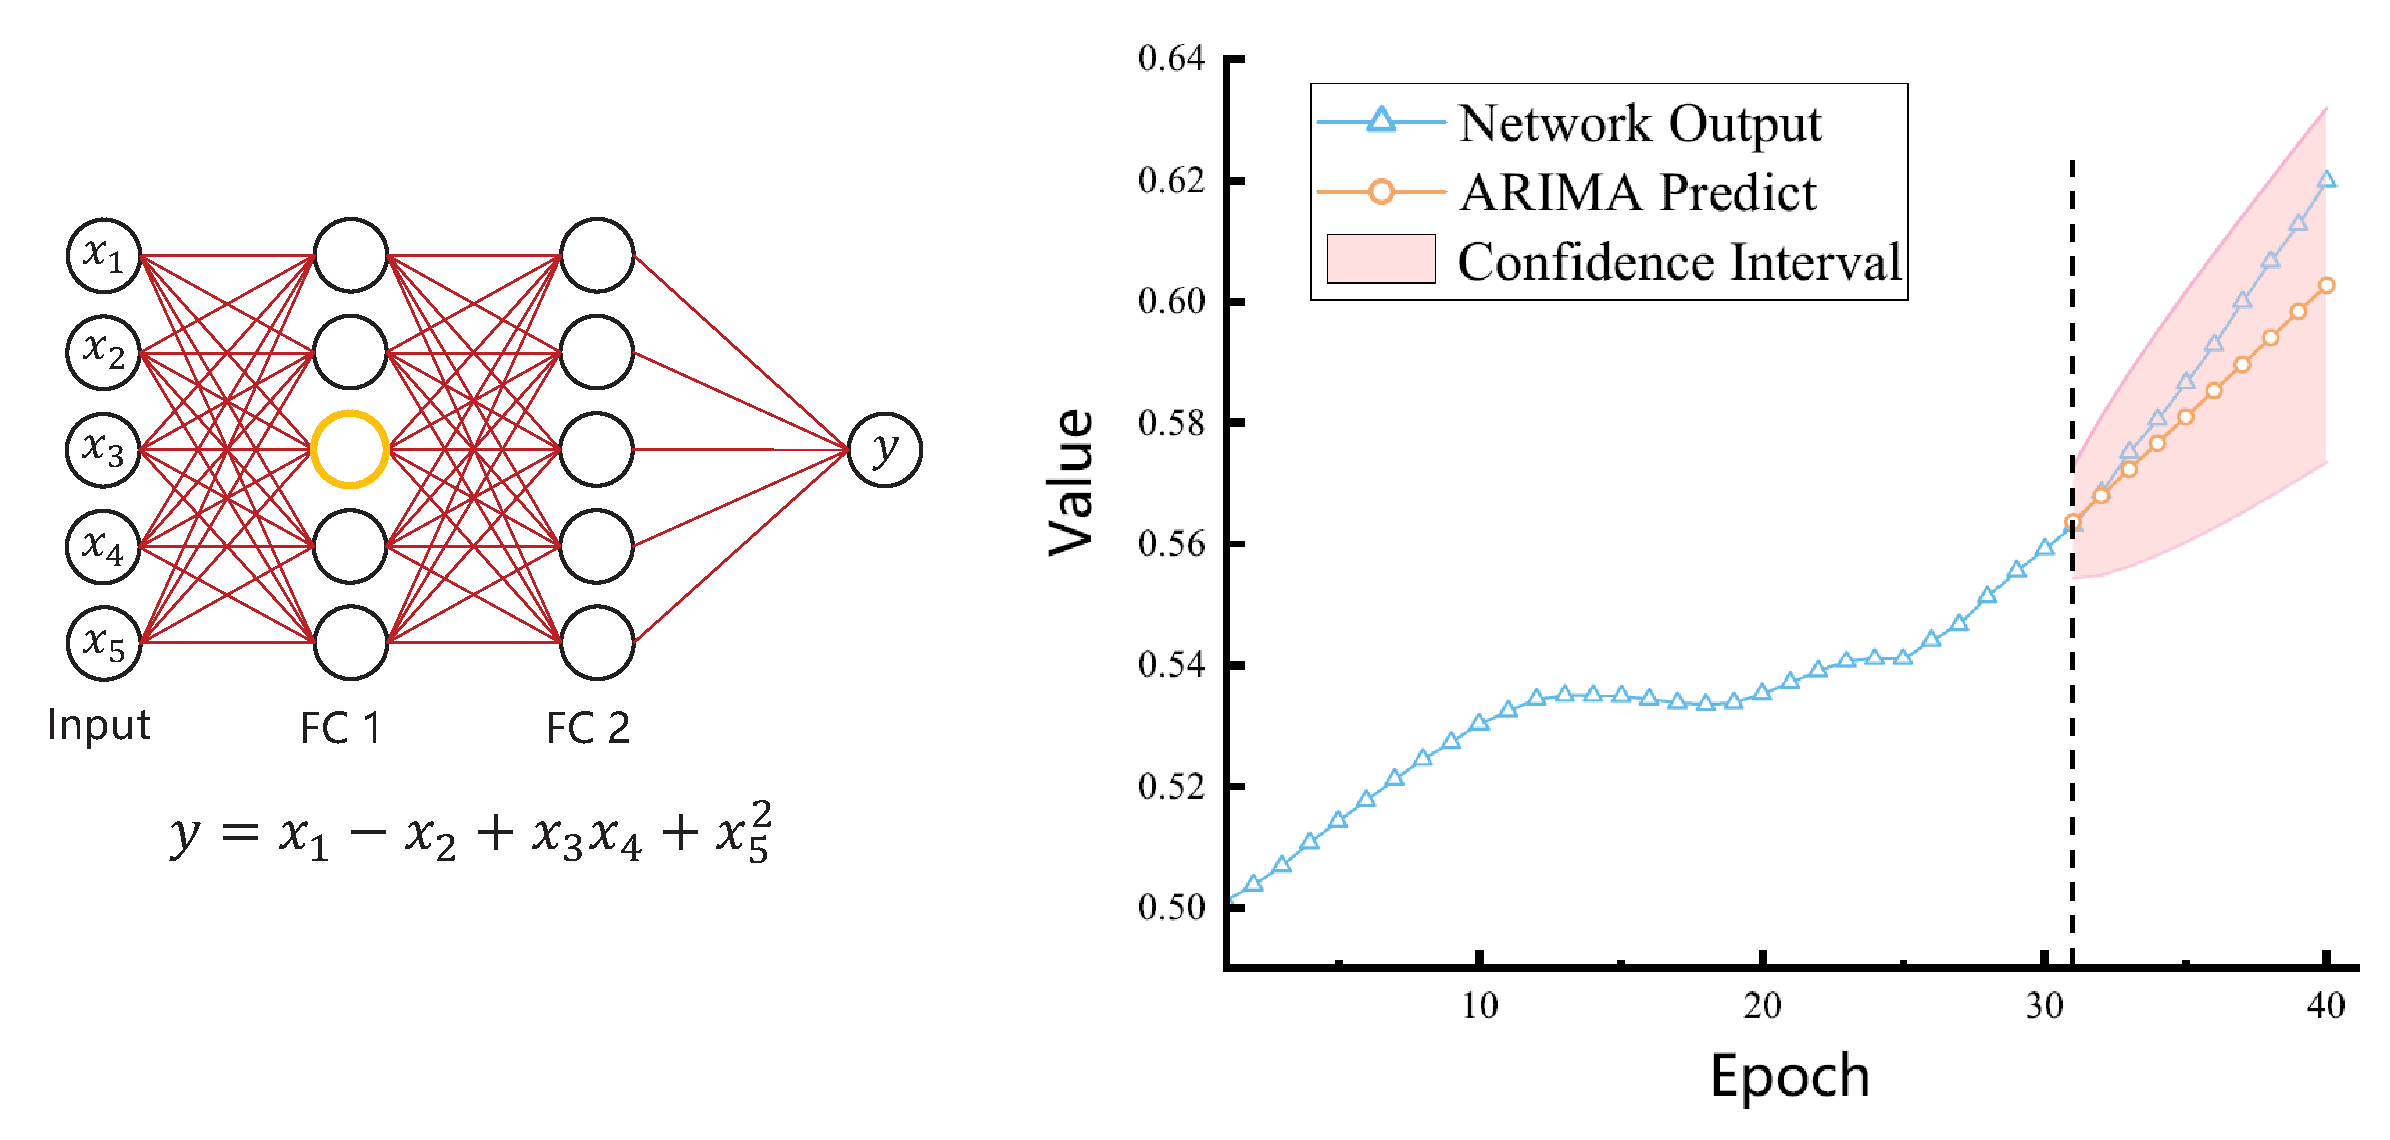
\includegraphics[scale=0.2]{figs/ARIMAv3.eps}
	\caption{The ARIMA analysis of the fully connected network. We record the output of a neuron in FC1 in the first 30 epochs, and use ARIMA to predict its output in the next 10 epochs. The results show that the prediction can match well with the real outputs. }
        \label{figintro}
\end{figure}
\begin{figure*}[htpb]
    \centering
    \subfigure[Classical KD]{
        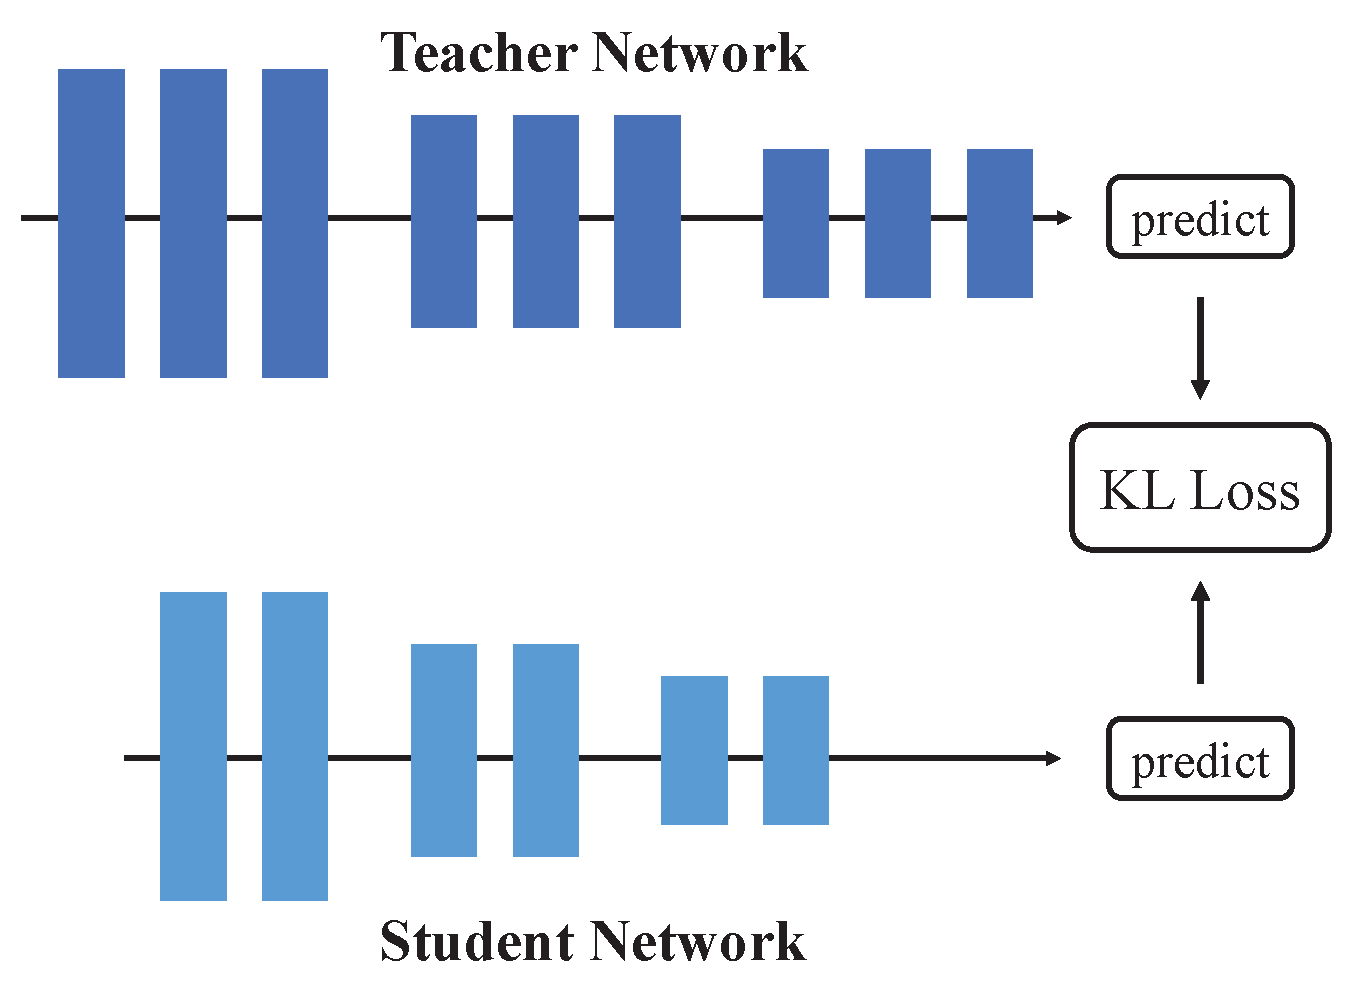
\includegraphics[scale = 0.22]{figs/general_KD.eps}}
    \subfigure[Feature-based KD]{
        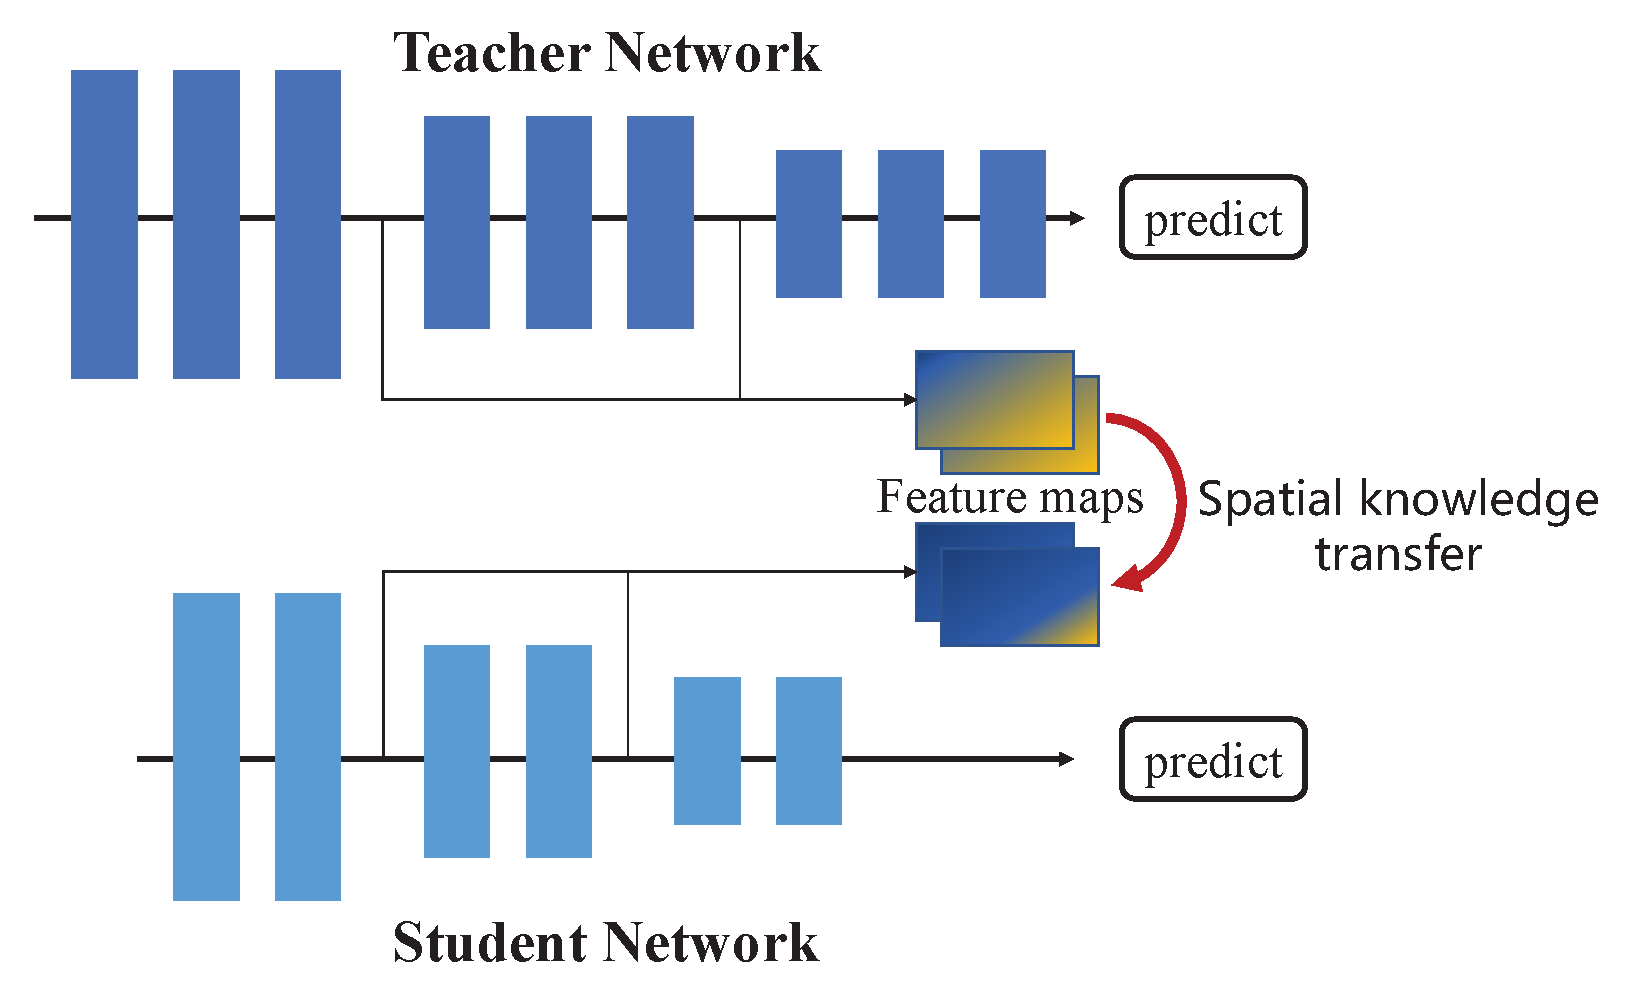
\includegraphics[scale = 0.22]{figs/feature_based_KD.eps}}
    \subfigure[Our TSKD]{
        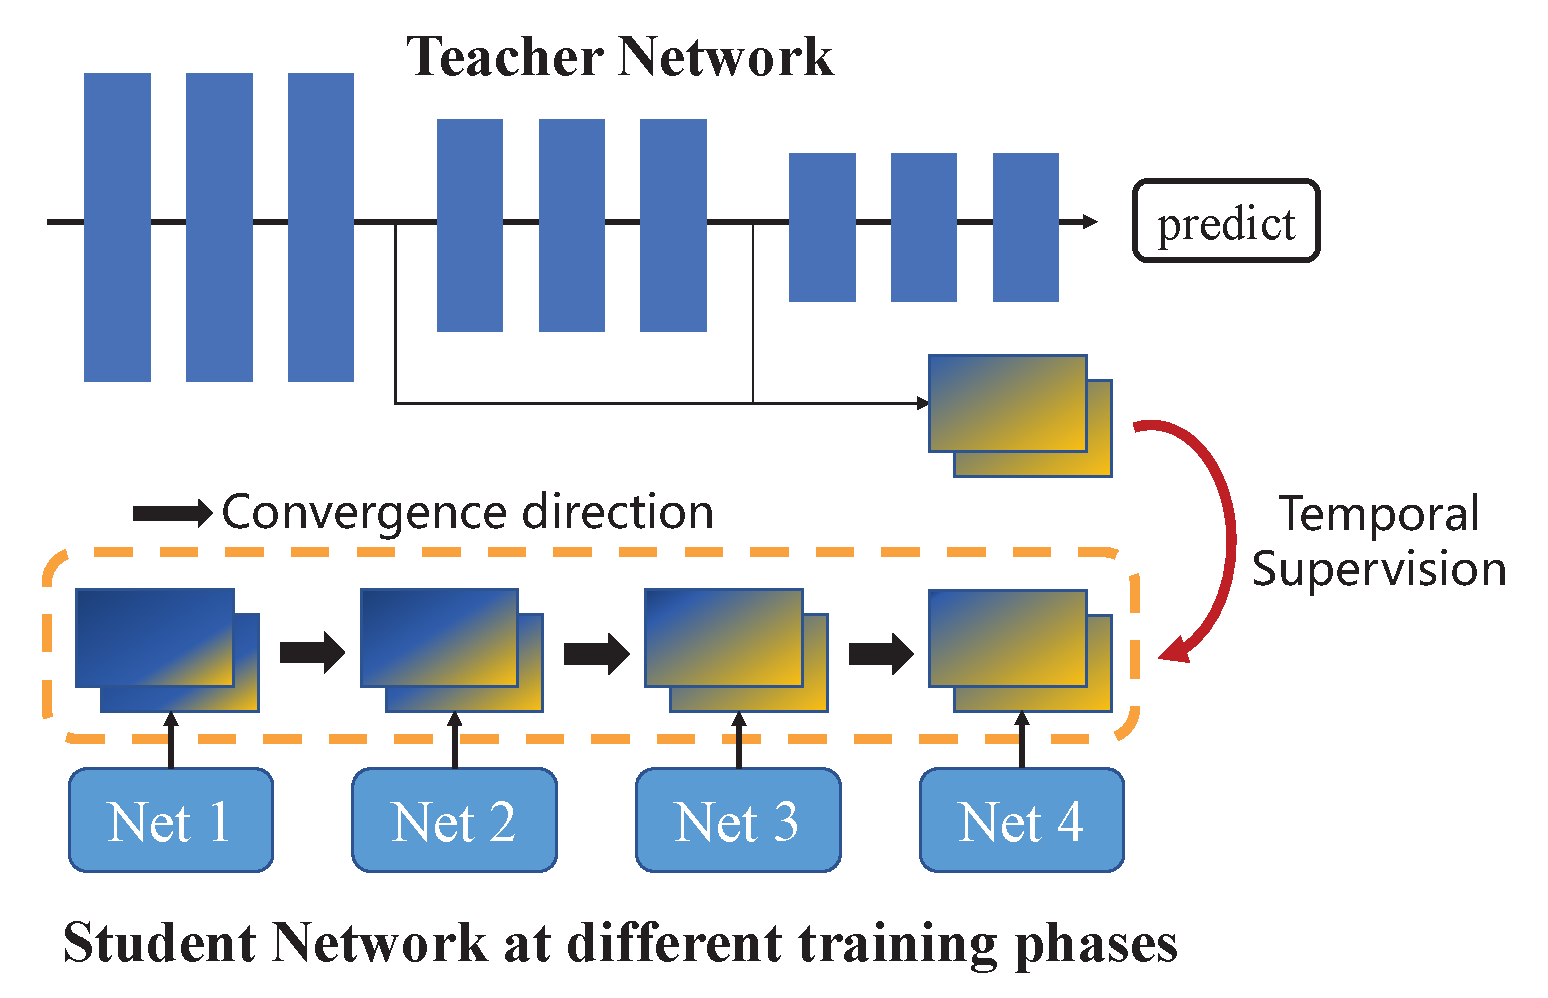
\includegraphics[scale = 0.22]{figs/TSKD2.eps}}
\caption{Illustration of classical KD, feature-based KD and our \textbf{TSKD}. Instead of distilling between corresponding Teacher-Student outputs, we aim to make teacher supervise the temporal learning process of student. }
    \label{fig2}
\end{figure*}
In this paper, we propose to distill along the temporal dimension. Our motivation comes from the human learning process, where \emph{reviewing} not only deepens our memory of old knowledge, but also more importantly, inspires us to learn the new knowledge. We believe that the learning process of neural networks also possesses strong temporal relationship.


To verify this hypothesis, we conduct time series prediction analysis on a fully connected network using Autoregressive Integrated Moving Average model (ARIMA) \cite{box1970distribution}. Specifically, we train the network to fit a quadratic function and use ARIMA to model the intermediate outputs through different epochs. As shown in Fig. \ref{figintro}, the fitted ARIMA model can provide an approximate prediction to the real training process, which indicates the temporal sequence property of network learning. Based on this discovery, we come up with two questions: (1) Can networks utilize the old knowledge to assist current learning like humans? (2) How to apply positive supervision to the temporal learning process of network?



To solve these two questions, we propose a novel knowledge distillation framework named \textbf{T}emporal \textbf{S}upervised \textbf{K}nowledge \textbf{D}istillation (TSKD). Different from existing feature-based distillation methods that distill knowledge from spatial features, we attempt to extract more knowledge along the temporal dimension (Fig. \ref{fig2}(c)). Firstly, we modify the student network training as a memorize-review mode, which imitates the human learning and reviewing knowledge. Moreover, we design a dynamic learning target with teacher features to train the temporal feature extractor, which enables teacher to guide the learning process of students. A powerful student network can be obtained by the temporal supervision of the teacher network.



Overall, our contributions are summarized as follows:

$\bullet$ We find that the knowledge in the network training grows regularly over time. There exists exploitable information in the temporal dimension.

$\bullet$ We establish a new training paradigm by planning the network training as memorize-review mode. This makes it possible for the student network to review old knowledge and utilize it to assist current learning.

$\bullet$ We propose a novel knowledge distillation framework by supervising the student network along the temporal dimension. Specifically, we use Conv-LSTM network to extract temporal features in the student learning and train it with a dynamic target.

$\bullet$ We achieve competitive performance against representative feature-based distillation works on various network architectures and different computer vision tasks.


\section{Related Work}
The concept of knowledge distillation was firstly proposed by Hinton \emph{et al.} in \cite{hinton2015distilling}. As an efficient manner to train smaller student networks with the guidance of bigger teacher networks, it is applied to various downstream tasks \cite{li2017mimicking, li2021online}.

Previous research mainly focus on matching the output distributions of two models \cite{hinton2015distilling,mirzadeh2020improved,cho2019efficacy,furlanello2018born}. As intermediate features contain more valuable information, FitNets \cite{romero2014fitnets} was proposed to transfer the knowledge from teacher network features to student network features using $\mathcal{L}_{2}$ distance as a constraint. Following FitNets, most of the research attention has been drawn to utilize the knowledge within intermediate features and feature-based methods have achieved state-of-the-art distillation performance. Representative works can be categorized to two branches: design new transformation and loss functions \cite{zagoruyko2016paying,tian2019contrastive,heo2019comprehensive}; optimize the matching relationship between teacher and student feature candidates \cite{chen2021distilling,ji2021show}


Most works distill between the corresponding teacher-student outputs directly. Though ReviewKD \cite{chen2021distilling} proposed to perform review in the distillation, its main idea is to utilize multi-level information of the teacher to guide one-level of the student, which realized multiscale spatial knowledge transfer. This paper focused on supervising the student along the temporal dimension.

\section{Method}

\subsection{Notations and definitions}
Let $S_{i}$ denote the student network at the $i$th training epoch and $T$ denote the teacher network. Given the same input data $X$, we denote the intermediate features of teacher layer $t_{l}$ and student layer $s_{l}$ as $F_{t_{l}}$ and $F_{s_{l}}^{i}$ respectively.
Previous works have mainly focused on transferring spatial knowledge from $F_{t_{l}}$ to $F_{s_{l}}^{i}$, usually by reducing the distance between the two in the transformation space. The adding loss term for $S_{i}$ can be written as follows:
\begin{align}
	\label{eq:1}
	L_{spatial} = \mathcal{D}\Big(Map(F_{s_{l}}^{i}),Map(F_{t_{l}})\Big)
\end{align}

\noindent where $Map(\cdot)$ is the transformation that transfers the feature map to a more representative space, and $\mathcal{D}(\cdot)$ is the distance measurement function. Similarly, multi-layers distillation is written as:
\begin{align}
	\label{eq:2}
	L_{spatial} = \sum_{(s_{l},t_{l})\in \mathcal{C}}\mathcal{D}\Big(Map(F_{s_{l}}^{i}),Map(F_{t_{l}})\Big)
\end{align}
where $\mathcal{C}$ stores the layers of features to transfer knowledge.
And the loss function of feature-based KD is:
\begin{align}
	\label{eq:2}
	L_{student} = L_{task} + \lambda L_{spatial}
\end{align}

\begin{figure*}[htbp]
	\centering
		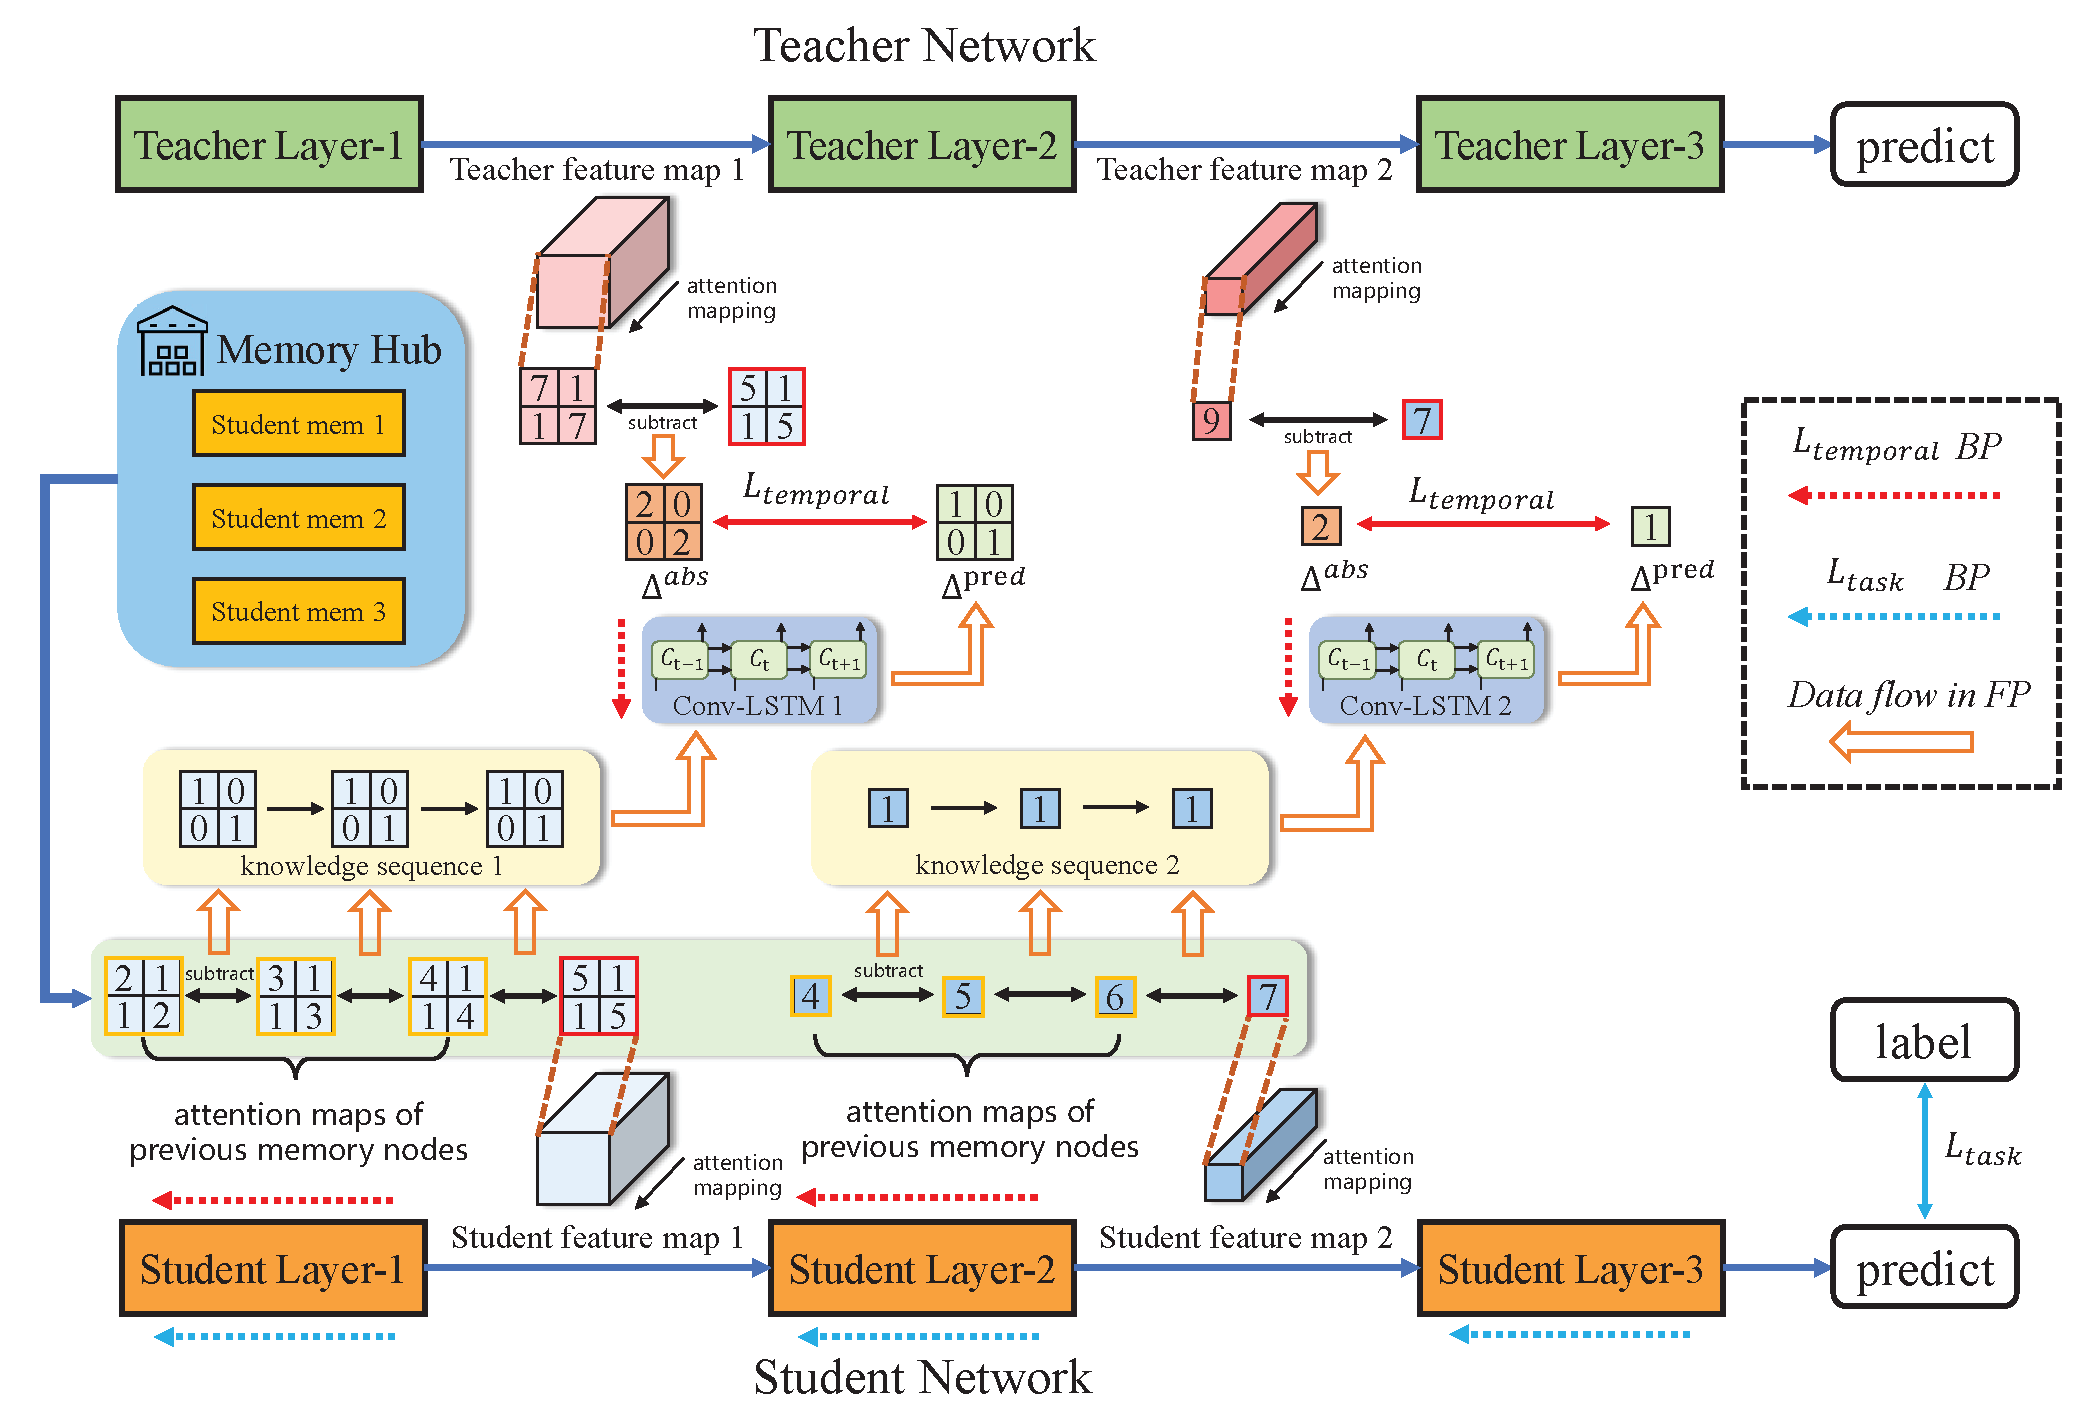
\includegraphics[scale=0.39]{figs/mainv4.eps}

	\caption{An overview of the proposed Temporal Supervised Knowledge Distillation (TSKD). During training at a review node, the same data will be input into the $k$ memory networks and the current student network. After transforming their outputs feature maps to attention maps, knowledge sequences are obtained by connecting the increments between two adjacency states. Finally, $\mathcal{L}_{temporal}$ is calculated between Conv-LSTM's prediction and the absolute increment. \emph{BP} and \emph{FP} denote back propagation and forward propagation respectively. }

 \label{fig3}
\end{figure*}
 The core idea is to use teacher features as auxiliary optimization goals. Although $L_{spatial}$ brings improvements to students, these methods neglect the progressive learning process. In our method, we exploit the temporal information in student learning and use the teacher model to guide the whole learning process.
Specifically, we view the training of the student network as a temporal process and plan it as a memorize-review mode (shown in Fig. \ref{fig4}). Here we give some definitions for better explaining our method. The replanned training is also shown more clearly in Algorithm \ref{alg:algorithm}.


\noindent\textbf{\emph{Action 1 (Memorize)}}: As the training progresses, the network will gradually converge. We hope that the network can memorize the current state at some points for future review. This action is implemented by saving the current model.

\noindent \textbf{\emph{Action 2 (Train)}}: This action is the same as the general data-based training and continues throughout the entire training process.

\noindent \textbf{\emph{Action 3 (Review)}}: Review the knowledge learned in $k$ previous memory nodes and utilize it to assist the current training. The implementation details are given in the following section.


\noindent \textbf{\emph{Memory nodes}}: Perform Action 1 and 2. The set of memory nodes is denoted by $\mathcal{M}$.

\noindent \textbf{\emph{General nodes}}: Only perform Action 2. The set of general nodes is denoted by $\mathcal{G}$.

\noindent \textbf{\emph{Review nodes}}: Perform Action 2 and 3.The set of review nodes is denoted by $\mathcal{R}$.

\noindent \textbf{\emph{Memory interval}}: The number of general nodes between memory nodes, denoted by $\delta$.

\begin{figure}[htbp]
	\centering
		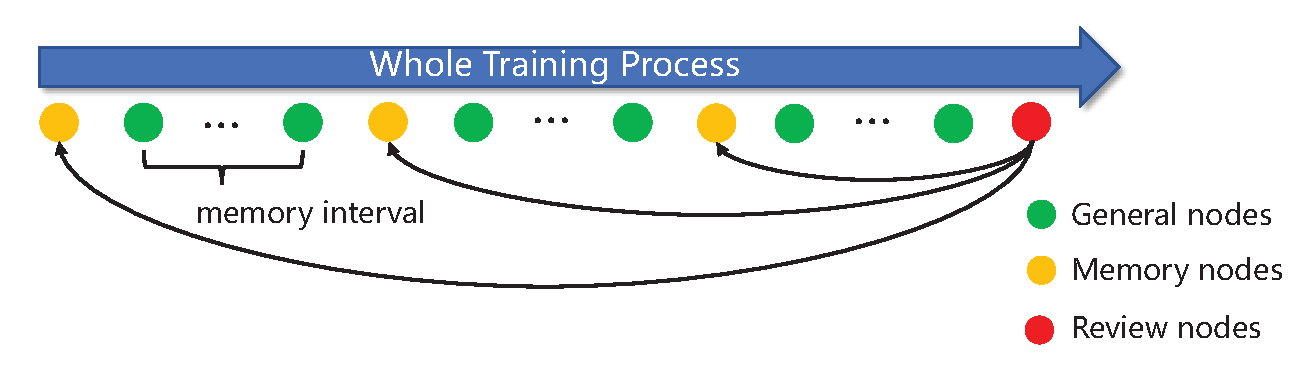
\includegraphics[scale=0.42]{figs/axis2.eps}
	\caption{The replanned training process. Each node corresponds to an epoch in training. }
        \label{fig4}
\end{figure}

\subsection{Review Mechanism}\label{subsec3.3}
Given input data $X$, the student model will have outputs at different layers, which contain plentiful knowledge. The outputs evolve as training progresses. For example, the network will gradually focus on the class discriminative regions, which is called attention in previous works \cite{zagoruyko2016paying,guo2023class}. Take layer $s_{l}$ as an example, the \emph{knowledge increment} between two temporally adjacent models $S_{i-1}$ and $ S_{i}$ can be represented as:
\begin{align}
    \Delta^{i-1,i}_{s_{l}} = \Big|Map(F_{s_{l}}^{i}) - Map(F_{s_{l}}^{i-1})\Big|
\end{align}

Intuitively, $\Delta^{i-1,i}_{s_{l}}$ represents the cognitive differences between $S_{i}$ and $S_{i-1}$ for the same input $X$.

When the training reaches a review node $S_{t},t\in\mathcal{R}$, we calculate increments among $k$ previous memory nodes and $S_{t}$, and connect them to obtain a length $k$ knowledge sequence:
\begin{align}
    knowledge\_seq = (\Delta^{t-k\delta,t-(k-1)\delta}_{s_{l}},\dots,\Delta^{t-\delta,t}_{s_{l}})
\end{align}


\noindent where $\delta$ denotes the memory interval. The value of $\delta$ indicates the number of general nodes between two memory nodes. As the knowledge sequence briefly summarizes the learning process during the period, we use a simple Conv-LSTM network to extract temporal features in it and obtain a prediction:
\begin{align}
    \Delta_{s_{l}}^{pred} = ConvLSTM(knowledge\_seq)
\end{align}

Specifically, the sequence can be seen as ``what has been learnt'' (old knowledge) in previous training, and Conv-LSTM gives a prediction of ``what to learn next'' based on the sequence. Now the problem is the training of the Conv-LSTM network. Due to the complexity of neural network and data distribution, it is hard to find an optimal solution for the whole learning process of student. However, we already have a well-trained teacher network whose outputs can be used as strong outlines. Thus, we design the following distillation mechanism. Specifically, we calculate the increment between $S_{t}$ and $T$ and use it as Conv-LSTM's target:
\begin{align}
    \Delta^{abs}_{s_{l},t_{l}} = \Big|Map(F_{t_{l}})-Map(F_{s_{l}}^{t})\Big|
\end{align}
We call $\Delta^{abs}_{s_{l},t_{l}}$ as absolute increment because it implies ``what needs to be learnt''. More importantly, $\Delta^{abs}_{s_{l},t_{l}}$ is a dynamic learning goal that changes as student outputs gradually approximate teacher outputs during training. This is more suitable for training in a memorize-review cycle.

In conclusion, for the current review node, the temporal loss can be calculated as :
\begin{align}
    L_{temporal} =  \Big\Vert \Delta_{s_{l}}^{pred} -\Delta^{abs}_{s_{l},t_{l}}\Big\Vert_{2}
    \label{eq8}
\end{align}
Similarly, equation \ref{eq8} can also be written in multi-layers style:
\begin{align}
    L_{temporal} = \sum_{(s_{l},t_{l})\in \mathcal{C}} \Big\Vert \Delta_{s_{l}}^{pred} -\Delta^{abs}_{s_{l},t_{l}}\Big\Vert_{2}
\end{align}
where $\mathcal{C}$ stores the layers of features to perform \emph{review}. The update of Conv-LSTM will also bring gradients to student based on chain rule , which can be represented as:
\begin{align}
    \theta_{S_{t+1}} = \theta_{S_{t}} - \alpha \frac{\partial L_{temporal}}{\partial \theta_{lstm}}\frac{\partial \theta_{lstm}}{\partial \theta_{S_{t}}},
\end{align}

 \noindent where $\theta_{S_{t}}$ and $\theta_{lstm}$ denote the parameters of student and Conv-LSTM respectively. The overall loss function of student network at a review node is:
\begin{align}
    L_{student} = L_{task} + \lambda L_{temporal}
\end{align}

To get a better understanding of our method, we provide detailed description in Fig. \ref{fig3} and Algorithm \ref{alg:algorithm}.
\begin{algorithm}[htpb]\small
\caption{Temporal Supervised Knowledge Distillation}
\label{alg:algorithm}
\textbf{Input}: A pre-trained teacher model with parameters $\theta_{t}$; A student model with initialized parameters $\theta_{s}$; A Conv-LSTM model with initialized parameters $\theta_{lstm}$; Training dataset $\mathcal{D}$;\\
\textbf{Initialization}: Set memory interval $\delta$; Divide the training into three nodes sets $\mathcal{M},\mathcal{G}$ and $\mathcal{R}$; \\
\textbf{Output}: A well-trained student model;

\begin{algorithmic}[1] %[1] enables line numbers
\WHILE{$\theta_{s} $ not converged}
\STATE Sample a mini-batch $\mathcal{B}$ from $\mathcal{D}$.
\IF {current node $\in$ $\mathcal{M}$}
\STATE Freeze $\theta_{lstm}$;
\STATE Perform general \emph{train} on $\mathcal{B}$ and update $\theta_{s}$ with $L_{task}$;
\STATE \emph{Memorize} the current state.
\ELSIF{current node $\in$ $\mathcal{G}$}
\STATE Freeze $\theta_{lstm}$;
\STATE Perform general \emph{train} on $\mathcal{B}$ and update $\theta_{s}$ with $L_{task}$.
\ELSIF{current node $\in$ $\mathcal{R}$}
\STATE Unfreeze $\theta_{lstm}$;
\STATE Forward propagation $\mathcal{B}$ into $\theta_{t}$ and $\theta_{s}$ to obtain $F_{t_{l}}$ and $F_{s_{l}}$ across layers;
\STATE Construct $knowledge\_seq$ and forward it into $\theta_{lstm}$ to obtain $\Delta^{pred}_{s_{l}}$, calculate $L_{temporal}$;
\STATE Update $\theta_{lstm}$ with $L_{temporal}$, update $\theta_{s}$ with $L_{task}$ and $L_{temporal}$,
\ENDIF
\ENDWHILE
\end{algorithmic}
\end{algorithm}

\noindent\textbf{Map function.} We choose Attention Transfer ($AT(\cdot)$) as map function in our method, which utilizes the insight of \cite{zagoruyko2016paying}. It is a transformation function that maps a 3D feature map tensor $F \in \mathbb{R}^{C\times H\times W}$ to a 2D attention map $F_{sum} \in \mathbb{R}^{H\times W}$. In our method, $F$ is flattened by summing the squares along the channel dimension, which can be denoted as:
\begin{align}
    F_{sum} = \textstyle \sum _{n=1}^{C}|F_{n}|^{2}
\end{align}
Although various transformation functions have been proposed \cite{tian2019contrastive, heo2019comprehensive} to map the features maps to a more knowledge-transferable space, we choose $AT(\cdot)$ because it is simple and intuitive. More importantly, it does not bring disruption to the temporal pattern contained in the original feature maps. The distribution of values in $F_{sum}$ reflects the spatial attention of the network clearly.
\\
\noindent\textbf{Temporal feature extractor.} In the proposed method, KD is reformulated as a time series prediction problem. Since ARIMA \cite{box1970distribution} can not deal with high-dimension data and transformer \cite{vaswani2017attention} may contribute to higher computational cost, we choose Conv-LSTM \cite{shi2015convolutional} as the temporal feature extractor.
Conv-LSTM is a variation of general LSTM, which replaces the element-wise operations in calculation by convolutional operations. Thus, Conv-LSTM is able to handle spatiotemporal data. The detailed information of the designed Conv-LSTM in TSKD is attached in supplement due to the page limit.



\section{Experiments}
\begin{table*}[htbp]
\centering
\begin{tabular}{@{}ccccccccc@{}}
\toprule
\multirow{4}{*}{\begin{tabular}[c]{@{}c@{}}Distillation\\ Mechanism\end{tabular}}
& Teacher & ResNet56   & ResNet32x4  & WRN40-2    & WRN40-2  & ResNet110  &VGG13\\ \cmidrule(l){2-8}
& acc     & 72.34      & 79.42       & 75.61      & 75.61    & 72.99   &74.64   \\ \cmidrule(l){2-8}
& Student & ResNet20   & ResNet8x4   & WRN16-2    & WRN40-1  & ResNet32   &VGG8    \\
& acc     & 69.06      & 72.50       & 73.26      & 71.98    & 71.14    &70.36      \\ \midrule
Logits   & KD      & 70.66          & 73.33          & 74.92          & 73.54          & 73.08      &72.98    \\ \midrule
\multirow{9}{*}{Spatial feature}
& FitNets  & 69.21          & 73.50           & 73.58          & 72.24          & 71.06     &71.02     \\
 & PKT     & 70.34          & 73.64          & 74.54          & 73.54          & 72.61     &72.88     \\
& RKD     & 69.61          & 71.90           & 73.35          & 72.22          & 71.82       &71.48   \\
 & CRD     & 71.16          & 75.51          & 75.48          & 74.14          & 73.48      &73.94   \\
& AT     & 70.55          & 73.44          & 74.08          & 72.77          & 72.31     &71.43     \\
& VID     & 70.38          & 73.09          & 74.11          & 73.30           & 72.61      &71.23    \\
& OFD     & 70.98          & 74.95          & 75.24          & 74.33          & 73.23      &73.95    \\
& SP      & 69.97         & 72.94           & 73.83          & 72.43         & 72.69     & 72.68   \\
& CC      & 69.63          & 72.97          & 73.56          & 72.21      & 71.48           & 70.71 \\
\midrule
\multirow{2}{*}{Temporal feature}    & TSKD    & \textbf{71.76} & \textbf{75.73} & \textbf{75.77} & \textbf{74.49} & \textbf{73.81} & \textbf{74.75} \\
& $\Delta$ & \textcolor[RGB]{0, 155, 0}{+2.7} &\textcolor[RGB]{0, 155, 0}{+3.23} &\textcolor[RGB]{0, 155, 0}{+2.51} &\textcolor[RGB]{0, 155, 0}{+2.51} &\textcolor[RGB]{0, 155, 0}{+2.67} &\textcolor[RGB]{0, 155, 0}{+4.39}\\
\bottomrule
\hspace*{\fill} \\
\end{tabular}
\caption{Top-1 accuracy of the student network on CIFAR-100. And $\Delta$ represents the performance improvement over the vanilla student.}
\label{cifar100samestyle}
\end{table*}

We evaluate our TSKD on various networks architectures e.g., VGG \cite{simonyan2014very}, ResNet \cite{he2016deep}, Wide ResNet \cite{zagoruyko2016wide} and MobileNet \cite{sandler2018mobilenetv2}. We compare TSKD with existing distillation methods of different categories: logits-based: KD \cite{hinton2015distilling}, DKD \cite{zhao2022decoupled}; spatial feature-based: FitNets \cite{romero2014fitnets}, PKT \cite{passalis2018probabilistic}, RKD \cite{park2019relational}, CRD \cite{tian2019contrastive}, AT \cite{zagoruyko2016paying}, VID \cite{ahn2019variational}, OFD \cite{heo2019comprehensive}, SP \cite{tung2019similarity}, CC \cite{peng2019correlation}, CAT-KD \cite{guo2023class} and ReviewKD \cite{chen2021distilling}.

\noindent\textbf{Hyperparameters.} The loss weight $\lambda$, the number of memory nodes $k$ and the memory interval $\delta$ are important hyper-parameters in the review stage. For image classification, we set $\lambda = 1,k=3$ and $\delta=5$. For object detection, we set $\lambda = 0.4, k=3$ and $\delta = 1$. The influence brought by the different settings of these hyperparameters are explored further in ablation studies.


\noindent\textbf{Datasets.} (1) CIFAR-100 \cite{krizhevsky2009learning} comprises of 50,000 training images, with 500 images per class, and 10,000 test images. (2) ImageNet \cite{deng2009imagenet} is considered the most challenging dataset for classification, offering 1.2 million images for training and 50,000 images for validation across 1,000 classes. (3) MS-COCO \cite{lin2014microsoft} is an 80-category general object detection dataset. The \texttt{train2017} and \texttt{val2017} contain 118k and 5k images respectively.

\noindent\textbf{Implementation Details.} Our implementation for CIFAR-100 and ImageNet strictly follows \cite{chen2021distilling, zhao2022decoupled}. Specifically, for CIFAR-100, we train all models for 240 epochs with batch size 128 and decay the learning rate by 0.1 for every 30 epochs after the first 150 epochs using SGD. The initial learning rate is set to 0.1. For ImageNet, we adopt the standard training process, which involves training the model for 100 epochs with batch size 256 and decaying the learning rate every 30 epochs (initial learning rate is 0.1).

For MS-COCO object detection, we take the most popular open-source report Detectron2\footnote{https://github.
com/facebookresearch/detectron2} as our strong baseline. We train the student models using the standard training policy following tradition \cite{wang2019distilling}.

For fairness, previous method results are either reported in previous papers or obtained using author-released codes with our training settings.

\subsection{Main Results}

\begin{table*}[t]
\centering
\begin{tabular}{@{}ccc|ccccc|cc|c@{}}

\multicolumn{3}{c|}{Distillation Mechanism} &\multicolumn{5}{c|}{Spatial feature} & \multicolumn{2}{c|}{Logits} &Temporal feature\\ \Xhline{1.5pt}
 & Teacher & Student & CRD    & AT     & OFD     & ReviewKD   & CAT-KD    & KD & DKD     & TSKD      \\ \hline
top-1   & 76.16   & 68.87  & 71.37 & 69.56  & 71.25  & \textbf{72.56}   & 72.24  & 68.58  & 72.05  & 72.22                \\
top-5   &92.86    & 88.76  & 90.41      &89.33        & 90.34       & 91.00       & \textbf{91.13}               &88.98     &91.05    &90.99  \\
\hspace*{\fill} \\
\end{tabular}
\caption{Top-1 and top-5 accuracy (\%) on the ImageNet validation. We set ResNet-50 as the teacher and MobileNet-V2 as the student.}
\label{R50tomobile}
\end{table*}
\begin{table*}[t]
\centering
\begin{tabular}{@{}ccc|ccccc|cc|c@{}}
\multicolumn{3}{c|}{Distillation Mechanism} &\multicolumn{5}{c|}{Spatial feature} & \multicolumn{2}{c|}{Logits} &Temporal feature\\ \Xhline{1.5pt}
 & Teacher & Student & CRD    & AT     & OFD     & ReviewKD   & CAT-KD    & KD & DKD     & TSKD        \\ \hline
top-1   & 73.31   & 69.75   & 71.17 & 70.69 & 70.81 & 71.61 & 71.26   & 70.66  & 71.70 & \textbf{71.90} \\
top-5   & 91.41   & 89.07   & 90.13      &90.01       &89.98       &90.51      & 90.45              &89.88   &90.41   & \textbf{90.76 }             \\
 \\
\end{tabular}
\caption{Top-1 and top-5 accuracy (\%) on the ImageNet validation.We set ResNet-34 as the teacher and ResNet-18 as the student.}
\label{r34tor18}
\end{table*}



\noindent\textbf{CIFAR-100 classification.} Table \ref{cifar100samestyle} presents the results on CIFAR-100. We have categorized previous works into different groups based on the main idea. In contrast, our method utilizes the spatiotemporal feature extracted in the training process. Our method achieves $3 \sim 5\%$ improvements on different teacher-student pairs, which strongly demonstrates the effectiveness of TSKD.

\noindent\textbf{ImageNet classification.} We also conducted additional experiments on ImageNet to further validate our approach. Specifically, we experimented with two distillation settings: from ResNet50 to MobileNet and from ResNet34 to ResNet18. The experimental results are reported in Table \ref{R50tomobile} and Table \ref{r34tor18}. Our method achieves competitive results. In the setting from ResNet34 to ResNet18, the gap between the student and the teacher had already been reduced to a very small value of 1.61 by the previous best method. Nevertheless, we were able to further reduce this gap to 1.41, resulting in a 12\% relative performance improvement.

\noindent\textbf{MS-COCO object detection.} In addition to classification, we also apply our method to object detection task. For this task, we distill the output features of the teacher and student's backbones, following a similar procedure as in the classification task. We use the best pre-trained models provided by Detectron2 as teachers.


However, we find that the number of epochs for training a classical detection network is relatively fewer compared to the classification networks (usually hundreds). This makes it difficult for deploying the memorize-review pipeline. Singly applying TSKD can hardly achieve outstanding performance. Thus, we introduce ReviewKD \cite{chen2021distilling} as our strong baseline to obtain satisfactory results. It can be observed that our TSKD brings a further boost to the AP metrics, even the performance of ReviewKD is relatively high.
\begin{table*}[!h]
\centering
\begin{tabular}{@{}cl|lccccc@{}}
        & Method                  & mAP            & AP50           & AP75           & AP1            & APm            & APs            \\ \Xhline{1.5pt}
Teacher & Faster R-CNN w/R101-FPN & 42.04          & 62.48          & 45.88          & 54.60          & 45.55          & 25.22          \\
Student & Faster R-CNN w/R18-FPN  & 33.26          & 53.61          & 35.26          & 43.16          & 35.68          & 18.96          \\
        & w/KD                    & 33.97(+0.61)          & 54.66          & 36.62          & 44.14          & 36.67          & 18.71          \\
        & w/FitNets               & 34.13(+0.87)          & 54.16          & 36.71          & 44.69          & 36.50          & 18.88          \\
        & w/FGFI                  & 35.44(+2.18)          & 55.51          & 38.17          & 47.34          & 38.29          & 19.04          \\
        & w/ReviewKD             & 36.75(+3.49)          & 56.72          & 34.00          & 49.58          & 39.51          & \textbf{19.42} \\
        & w/ours+ReviewKD                 & \textbf{36.82(+3.56)} & \textbf{56.85} & \textbf{39.70} & \textbf{49.63} & \textbf{39.73} & 19.20          \\ \hline
Teacher & Faster R-CNN w/R101-FPN & 42.04          & 62.48          & 45.88          & 54.60          & 45.55          & 25.22          \\
Student & Faster R-CNN w/R50-FPN  & 37.93          & 58.84          & 41.05          & 49.10          & 41.14          & 22.44          \\
        & w/KD                    & 38.35(+0.42)          & 59.41          & 41.71          & 49.48          & 41.80          & 22.73          \\
        & w/FitNets                 & 38.76(+0.83)          & 59.62          & 41.80          & 50.70          & 42.20          & 22.32          \\
        & w/FGFI                  & 39.44(+1.51)          & 60.27          & 43.04          & 51.97          & 42.51          & 22.89          \\
        & w/ReviewKD              & 40.36(+2.43)          & 60.97          & 44.08          & 52.87          & 43.81          & 23.60          \\
        & w/ours+ReviewKD                  & \textbf{40.65(+2.72)} & \textbf{61.23} & \textbf{44.43} & \textbf{53.38} & \textbf{43.91} & \textbf{23.81} \\ \hline
Teacher & Faster R-CNN w/R50-FPN  & 40.22          & 61.02          & 43.81          & 51.98          & 43.53          & 24.16          \\
Student & Faster R-CNN w/MV2-FPN  & 29.47          & 48.87          & 30.90          & 38.86          & 30.77          & 16.33          \\
        & w/KD                    & 30.13(+0.66)          & 50.28          & 31.35          & 39.56          & 31.91          & 16.69          \\
        & w/FitNets                 & 30.20(+0.73)          & 49.8           & 31.69          & 39.69          & 31.64          & 16.39          \\
        & w/FGFI                  & 31.16(+1.69)          & 50.68          & 32.92          & 42.12          & 32.63          & 16.73          \\
        & w/ReviewKD              & 33.71(+4.24)          & 53.15          & 36.13          & \textbf{46.47} & 35.81          & 16.77          \\
        & w/ours+ReviewKD                  & \textbf{34.03(+4.56)} & \textbf{53.67} & \textbf{36.33} & 45.72          & \textbf{36.53} & \textbf{18.03}
\end{tabular}

\caption{Results on object detection. We use AP on different settings to evaluate results. R101 represents using ResNet-101 as backbone, and MV2 stands for MobileNetV2.}
\label{objection}
\end{table*}

\subsection{Ablation Studies}
\textbf{Feature maps as knowledge sequence}. In our distillation method, we extract spatiotemporal features from the increment sequence rather than feature map sequence. The reason we choose the increment is that it can filter the irrelevant information in feature maps. The network will pay more attention to the new content in the progressive learning.  The experiments show that using feature maps themselves as sequences also brings improvements, but increment groups have better performance (Table \ref{tab5}). In fact, first-order differential is a common way to process raw data in classical time series analysis problem, which will enhance the temporal property of the sequence. The experimental results are consistent with this theory.
\begin{table}[htbp]
\centering
\begin{tabular}{@{}c|cc@{}}
 T-S Structure  & fm. seq & inc. seq
\\ \Xhline{1.5pt}
 ResNet-56 to ResNet-20 & 71.19 &\textbf{71.76}
\\ \hline
 WRN40-2 to WRN40-1 &74.30 &\textbf{74.49}
\end{tabular}
\caption{Comparison results on different types of sequence. incre. and fm. denote increment and feature map respectively. }
\label{tab5}
\end{table}

\noindent\textbf{Effects of memory interval.} The memory interval $\delta$ determines how many epochs of general training are performed between memory nodes. When $\delta$ is relatively high, the learning period recorded in the knowledge increment sequence will become longer. This may make the review more difficult. Different settings of $\delta$ are explored in Table \ref{tab6}.
\begin{table}[htbp]
\centering
\begin{tabular}{@{}c|cc@{}}
 Interval $\delta$ & ACC($\%$)
\\ \Xhline{1.5pt}
 5 &\textbf{71.76(+2.70)}
\\ \hline
10 &71.28(+2.22)
\\ \hline
15 &71.19(+2.13)
\end{tabular}
\caption{Ablation studies on memory interval $\delta$ on CIFAR-100. The student and teacher models are ResNet-56 and ResNet-20 respectively. }
\label{tab6}
\end{table}

\noindent\textbf{Effects of memory nodes.} In order to investigate how many memory nodes are proper in one review, we compare different settings of $k$ in Table \ref{tab7}. Obviously, the knowledge sequence will become longer as the number of memory nodes increases. However, given the same training time, the frequency of review will also decrease accordingly. On the other hand, too few memory nodes can also make the temporal property in the sequence not clear enough. The R56-R20 experiment shows the highest accuracy when $k=6$.
\begin{table}[htbp]
\centering
\begin{tabular}{@{}cc|cccccc@{}}
& Value of $k$ & ACC($\%$)
\\ \Xhline{1.5pt}
& 3 &71.76(+2.70)
\\ \hline
&6 &\textbf{71.81(+2.75)}
\\ \hline
&9 &71.78(+2.72)
\end{tabular}
\caption{Ablation studies on the number of memory nodes on CIFAR-100. The student and teacher models are ResNet-56 and ResNet-20 respectively.}
\label{tab7}
\end{table}

\subsection{Extensions}
\noindent \textbf{Visualizations.} We visualize the deep features of student network WRN-16-2 (distilled from WRN-40-2 on CIFAR-100). The t-SNE (Fig. \ref{fig5}) results show that representations of TSKD are more separable than general KD, which proves that student trained by TSKD benefits from the discriminability of features.


\begin{figure}[htpb]
	\centering
	\begin{subfigure}
		\centering
		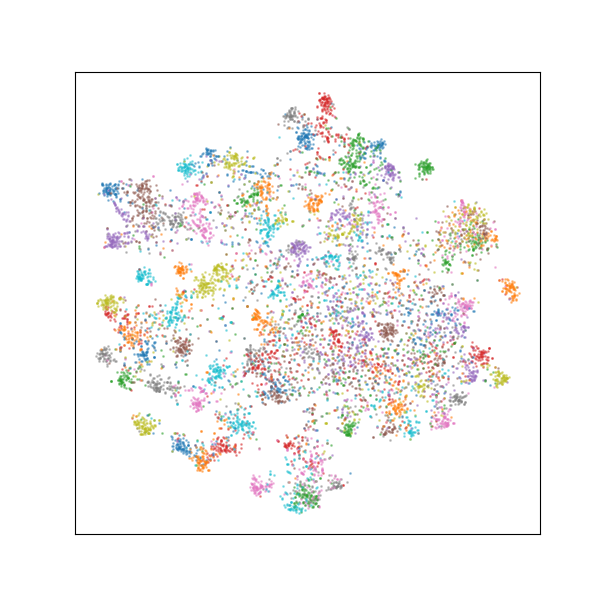
\includegraphics[scale=0.25]{figs/wrn_162_kl_half2_tsne.png}
	\end{subfigure}
	\begin{subfigure}
		\centering
		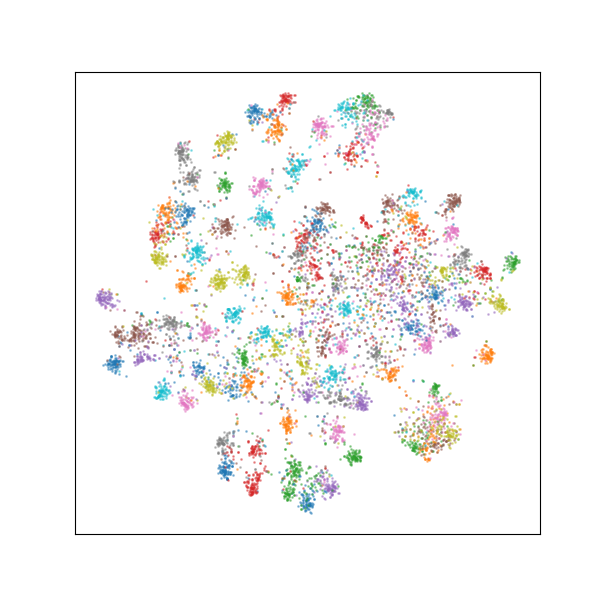
\includegraphics[scale=0.25]{figs/wrn_162_lstm_tsne.png}
	\end{subfigure}
\caption{t-SNE of features learned by KD (left) and TSKD (right). }
\label{fig5}
\end{figure}

\noindent \textbf{Efficiency.}
We compare the training cost of the proposed TSKD with state-of-the-art feature-based distillation methods. Specifically, we record the average training time per batch in a whole memory-review cycle. Different from existing methods which perform distillation throughout the entire training process, our TSKD, instead, only needs to distill in review nodes. Therefore, the computational costs of training student networks have been reduced. As the results reported in Fig. \ref{fig5}, our method has better trade-off between training time and accuracy.

\begin{figure}
    \centering
    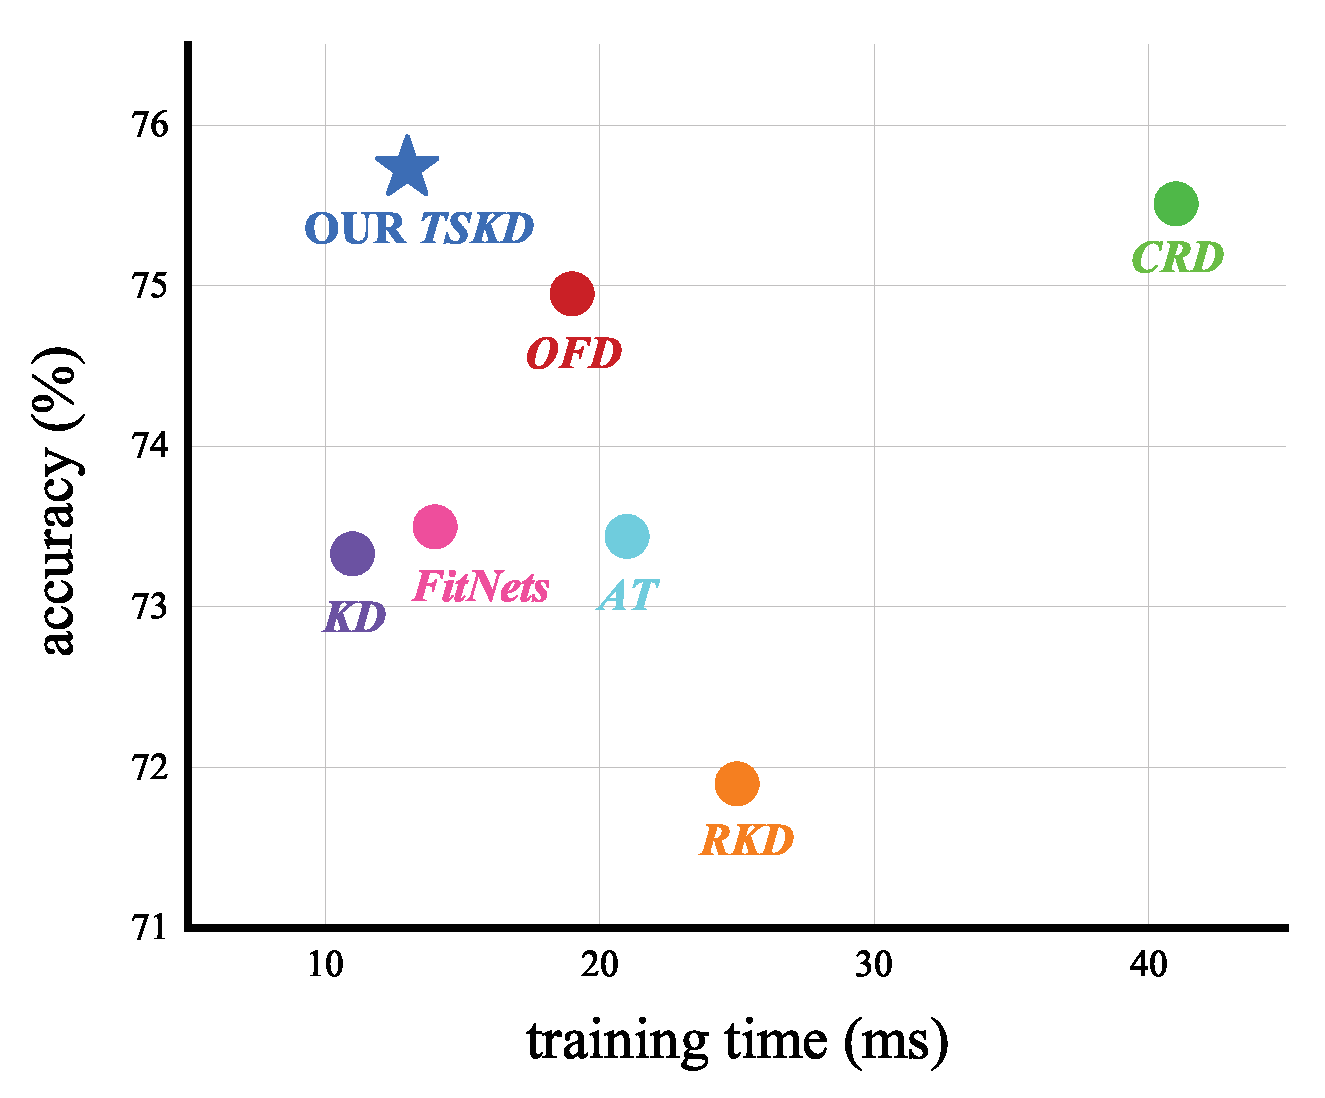
\includegraphics[scale = 0.24]{figs/efficiencyv2.eps}
    \caption{Training time (per batch) vs. accuracy on CIFAR-100. We set ResNet32x4 as the teacher and ResNet8x4 as the student. }
    \label{fig6}
\end{figure}


\noindent \textbf{Transferability.} We evaluate the generalizability of distilled student network. A primary goal of representation learning is to acquire general knowledge that is not only useful in the current dataset, but also in dataset/tasks from other domains. Therefore, we test if the knowledge distilled by TSKD transfer well. In the experiment, we use WRN-16-2 as the frozen representation extractors, which is either trained from scratch on CIFAR-100 or distilled from WRN-40-2 with various KD methods. We then perform linear probing tasks on TinyImageNet\footnote{https://www.kaggle.com/c/tiny-imagenet}. As the results reported in Table \ref{tab8}, TSKD outperforms other methods by a certain margin, demonstrating its strong generalizability.
\begin{table}[htpb]\small
\centering
\begin{tabular}{@{}c|cccccc@{}}
 baseline & KD & FitNets & CRD & ReviewKD & DKD &TSKD
\\ \Xhline{1.5pt}
 33.7 &33.9 &33.5 &35.6 &36.6 &37.1 &\textbf{38.5}

\end{tabular}
\caption{Comparison with previous methods on transferring representations from CIAFR-100 to TinyImageNet. }
\label{tab8}
\end{table}
\section{Conclusion}
This paper deals with the problem of knowledge distillation from a novel perspective. We find that there exists temporal pattern in the evolution of network knowledge. Motivated by this observation, we propose Temporal Supervised Knowledge Distillation (TSKD) to solve two questions: (1) How to utilize the old knowledge to assist current learning? and (2) How to supervise the temporal learning process of network? The student trained by TSKD achieves significant improvements on CIFAR-100, ImageNet and MS-COCO datasets for image classification and object detection tasks.
Besides, TSKD also shows superiority on training efficiency and knowledge transferability. We hope our work will help future research on knowledge distillation and interpretable deep learning.



Nulla eligendi quae odit, quidem at molestias autem error quaerat asperiores provident deserunt hic, ipsum delectus aliquid dignissimos ad animi numquam quaerat quo beatae natus, velit architecto blanditiis id consequuntur alias aut voluptatibus quas aspernatur vel iusto, officiis neque incidunt repudiandae iure aliquam ipsa quam.Recusandae totam harum provident accusamus iste debitis velit, dignissimos sapiente magni animi modi neque nihil, quo accusantium facilis autem voluptate nemo aliquid officia asperiores officiis sequi adipisci, asperiores sunt itaque ullam facilis delectus odio rem sint nihil?Accusantium quisquam similique ad perspiciatis harum, odio error debitis facere molestiae omnis, amet quod pariatur odio vero commodi a soluta rem accusantium aperiam totam, consectetur dolorum expedita porro nostrum, eveniet excepturi eos eaque repudiandae id.\clearpage
\bibliography{aaai24}

\end{document}